\section{Background of Vapor Intrusion}

\begin{frame}
  \frametitle{What is Vapor Intrusion?}
  \begin{figure}
    \centering
    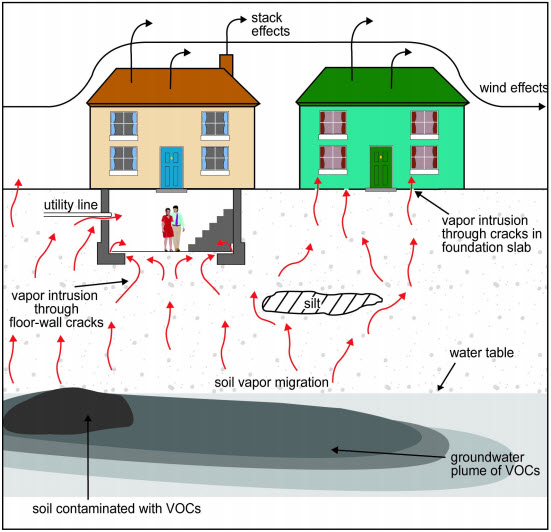
\includegraphics[width=0.7\textwidth]{vaporintrusion.jpg}
    \caption{\tiny{EPA\cite{us_epa_what_2015}}}
  \end{figure}
\end{frame}

\begin{frame}
  \frametitle{Why Should Vapor Intrusion Concern Us?}
  \begin{columns}[T]
    % text column
    \begin{column}{0.5\textwidth}
      \begin{block}{VI Contaminants}
        \begin{itemize}
          \item Volatile organic compounds (VOCs)
          \item Chlorinated organic solvents
          \begin{itemize}
            \item Trichloroethylene (TCE) (\SI{2}{\micro\gram\per\metre\cubed})
            \item Tetrachloroethylene (PCE)
          \end{itemize}
          \item Most of these carcinogenic
          \item Common at Superfund sites - one site may affect many buildings
        \end{itemize}
      \end{block}
    \end{column}
    % figure column
    \begin{column}{0.5\textwidth}
      \begin{figure}
        \centering
        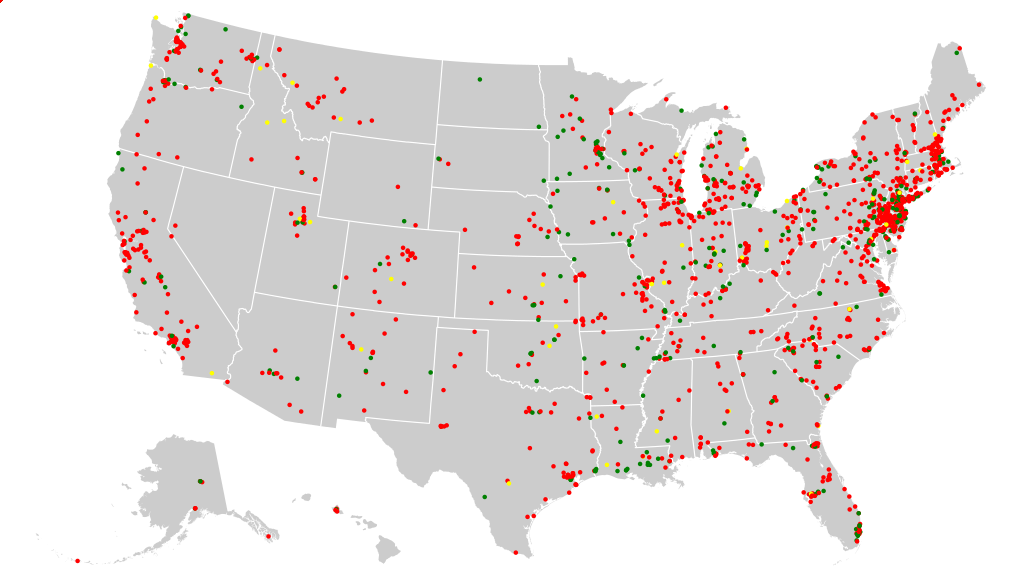
\includegraphics[width=\textwidth]{Superfund_sites.svg.png}
        \caption{Superfund sites as of 2013. \tiny{Wikipedia CC\cite{skew-t_filesuperfund_nodate}}}
      \end{figure}
    \end{column}
  \end{columns}
\end{frame}

% VI investigations
\begin{frame}
  \frametitle{Difficulties in VI Investigations}
  \begin{block}{Human concerns}
    \begin{itemize}
      \item Liability issues - responsible party
      \item Intrusive \& expensive
    \end{itemize}
  \end{block}
  \begin{block}{Practical concerns}
    \begin{itemize}
      \item Concern for indoor sources (false positives)
      \item VI sites affected by great variability (false negatives)
      \begin{itemize}
        \item Spatially
        \item Temporally
      \end{itemize}
      \item Requires multiple-lines of evidence (MLE) - spatially and temporally separated samples
    \end{itemize}
  \end{block}
\end{frame}


\begin{frame}
  \frametitle{Attenuation Factors and Empiricism}

\begin{columns}[T]
  \begin{column}{0.5\textwidth}
    \begin{block}{Determining VI}
      \begin{itemize}
        \item Decrease in vapor concentration from point to point - \textit{attenuation}
        \item Compare to EPA VI database recommended values ($\alpha_\mathrm{gw} \approx 0.001$)
        \item Does not capture individual site differences - highly empirical approach
        \item Need to make sense of complex data
      \end{itemize}
    \end{block}
  \end{column}

  \begin{column}{0.5\textwidth}
    \begin{block}{Attenuation factor}
      \centering
      $\alpha_\mathrm{gw} = \frac{c_{in}}{c_\mathrm{gw}}$\\
      \begin{figure}
        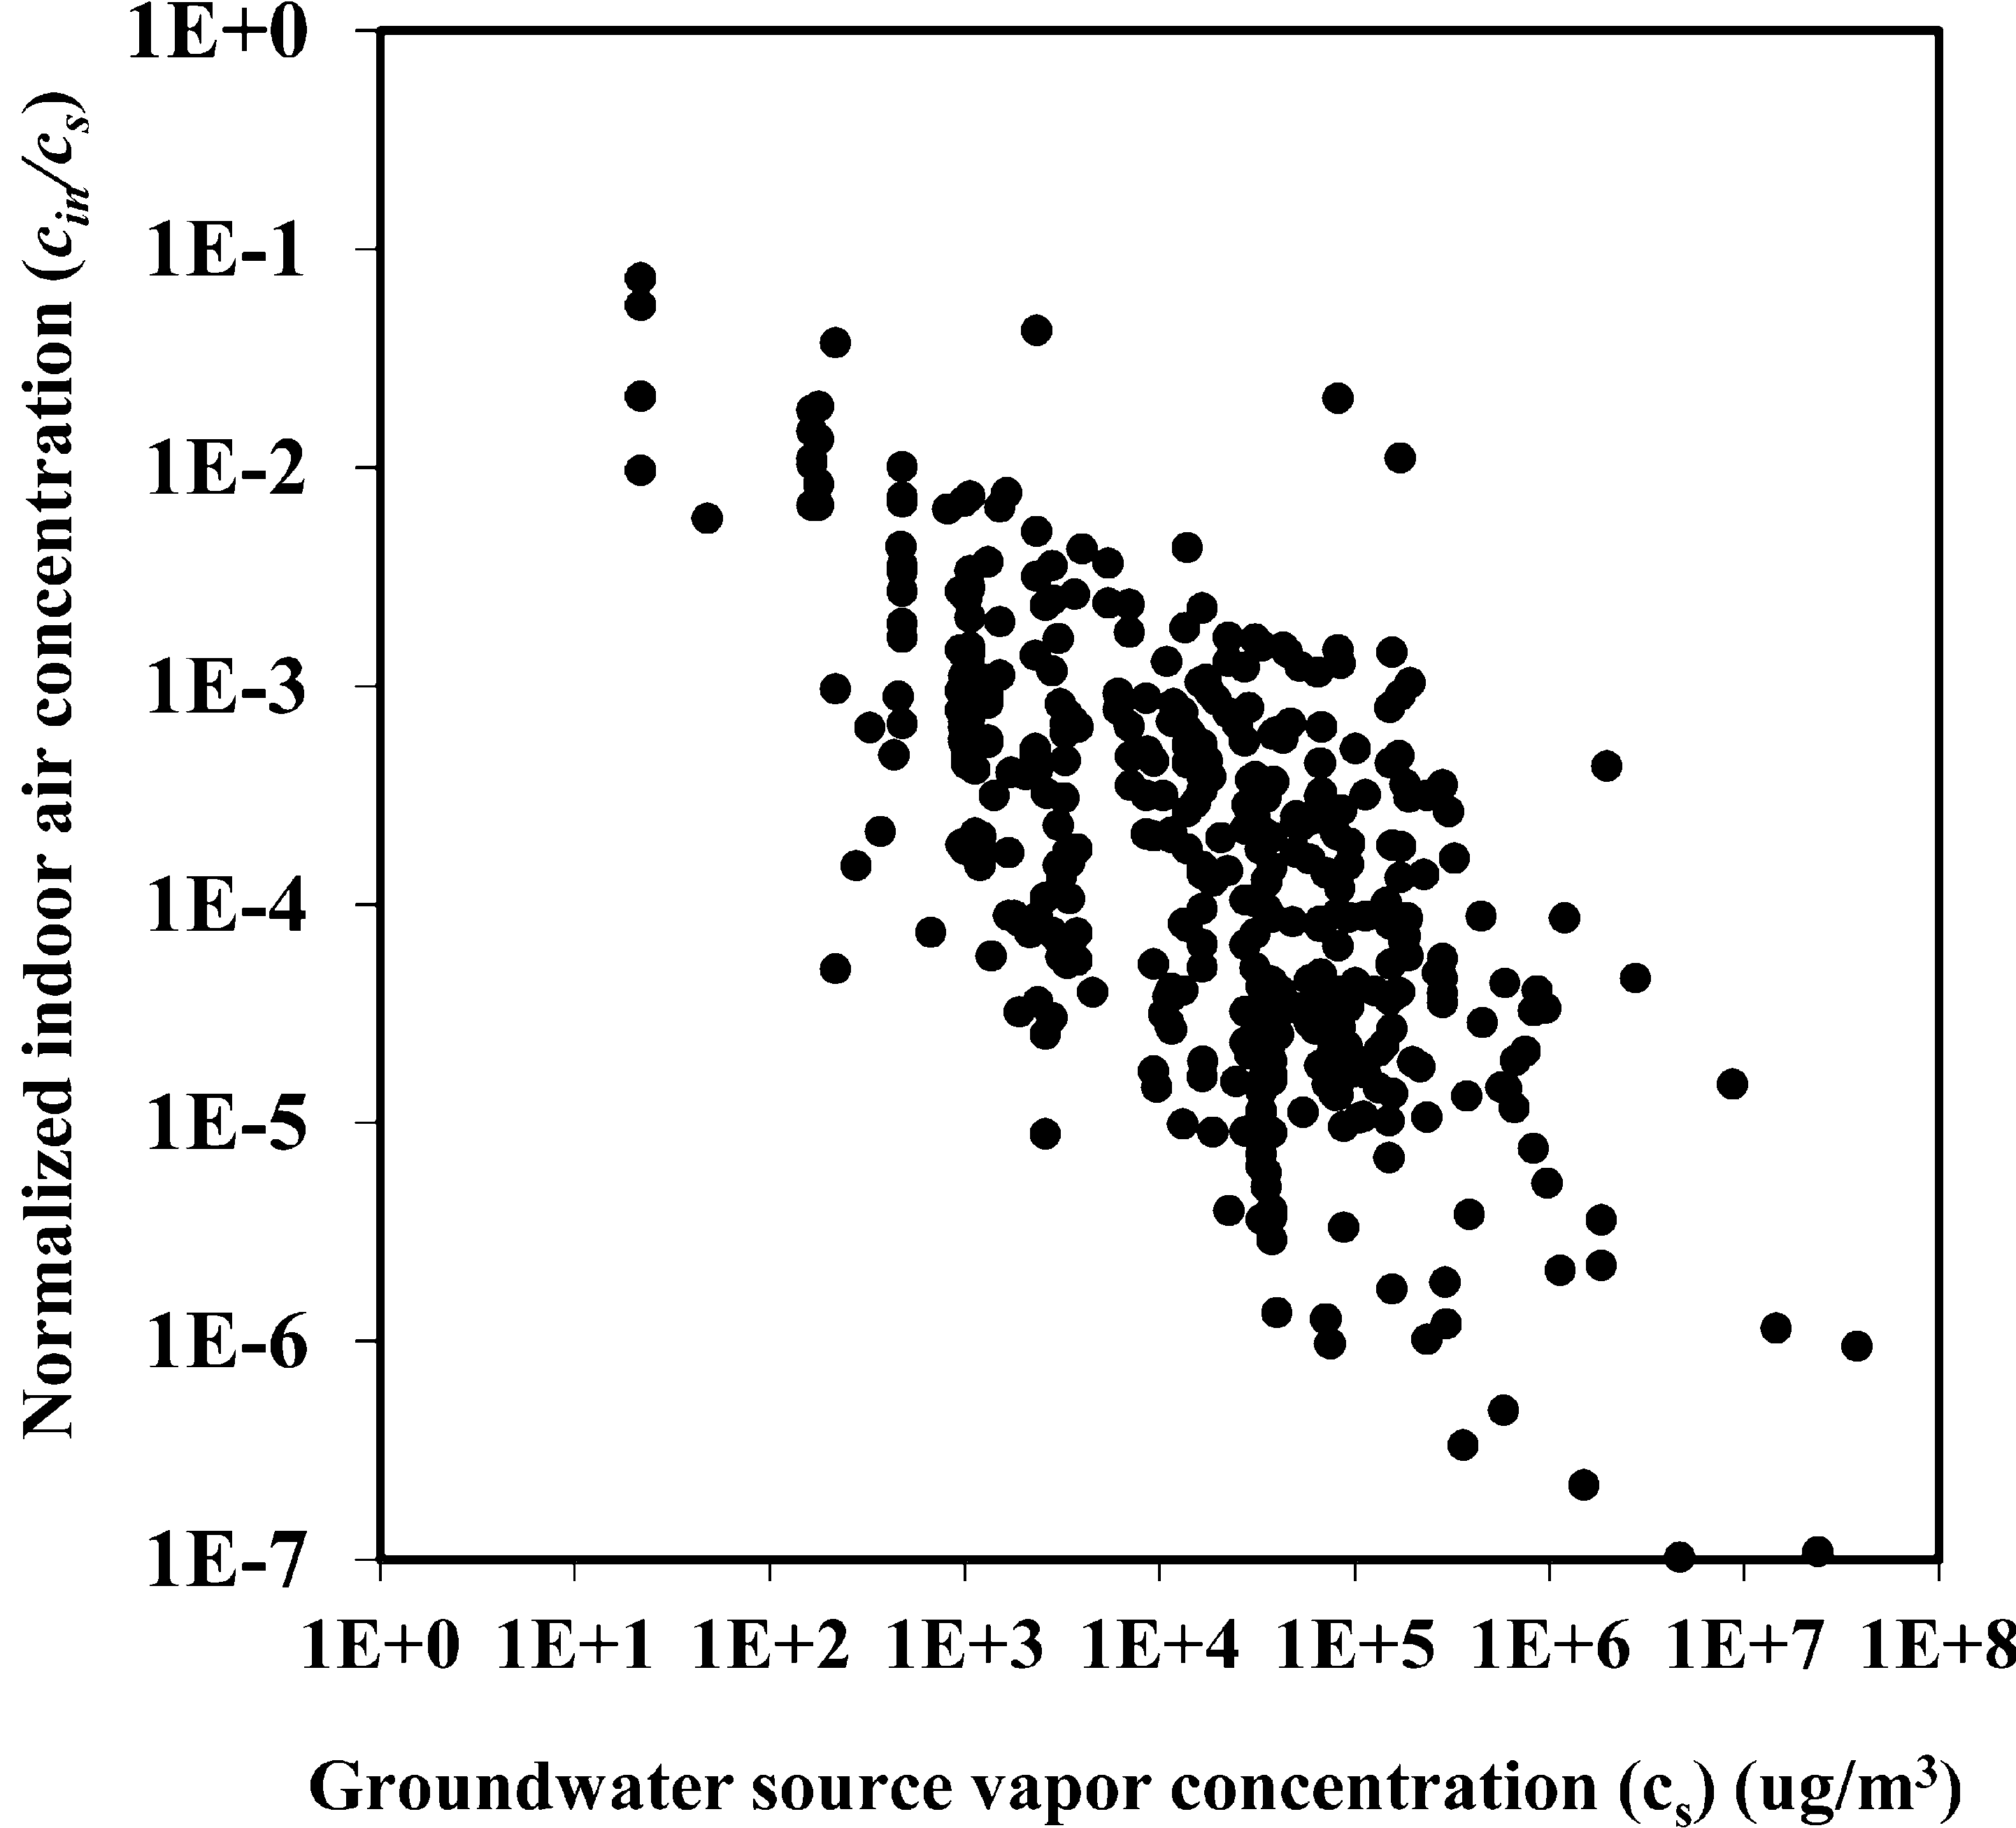
\includegraphics[width=\textwidth]{yao_attenuation.png}
        \caption{\tiny{\citeauthor{yao_examination_2013-1}\cite{yao_examination_2013-1}}}
      \end{figure}
    \end{block}
  \end{column}
\end{columns}
\end{frame}

\begin{frame}
  \frametitle{Benefits of Modeling in VI}
  \begin{block}{Advance Scientific Understanding}
    \begin{itemize}
      \item Can control for any variable/feature
      \item First-principles explanation of VI - discover new insights
      \item Hypothetical scenarios
    \end{itemize}
  \end{block}
  \begin{block}{Predictive Tool}
    \begin{itemize}
      \item Guide VI investigations
      \item Evaluate results
    \end{itemize}
  \end{block}
\end{frame}



\begin{comment}

\begin{frame}
  %\frametitle{Talk at a Glance}
  \begin{alertblock}{Key points}
    \begin{itemize}
      \item VI field is very empirical - need to make sense of complex field data \& consider site specific features
      \item Numerical models are a crucial tool for understanding vapor intrusion and generalizing conclusions
      \item Explain observed behavior of the "ASU house" vapor intrusion site
      \item Broader implications of these findings (and expand on these)
    \end{itemize}
  \end{alertblock}
\end{frame}


\begin{frame}
  \frametitle{Perspective on Indoor Air Quality}
  \begin{block}{Indoor air quality more relevant than ever}
    \begin{itemize}
      \item We spend up to 90\% of our time indoors\cite{klepeis_national_2001}
      \item Increased number of hazardous contaminants over time
      \item Sources inside the home (combustion particulates, mold, asbestos, etc.)
      \item External sources:
      \begin{itemize}
        \item Radon intrusion (1970s)
        \begin{itemize}
          \item Carcinogenic - generated by decay of U in soils \& rocks
          \item Significant accumulation of gas in indoor environment
          \item \nth{2} leading cause of lung cancer
        \end{itemize}
        \item Vapor intrusion (1990s)
        \begin{itemize}
          \item Broader - encompasses many anthropogenic contaminants
          \item Point source (spill) - groundwater dispersion
        \end{itemize}
      \end{itemize}
    \end{itemize}
  \end{block}
\end{frame}


Recommended $\alpha$ approach reveals a greater issue in VI investigations - a far too large emphasis on empirical analysis of results without really considering site specific conditions.

Empirical approach makes it difficult to:
- generalize any findings to other sites (sites are too varied and data too complex to easily unravel)
- too conservative for assessment

We need a way to make sense of the data from specific sites, to understand what specific conditions lead to the observed behavior.
This is achievable through first-principles numerical models. Allows us to:
  - replicate conditions at a site and control features
  - conversely can be used to predict VI based on site specific conditions

In this work we will show the use of such a model can be used to explain the observed behavior at well-studied VI site.
Specifically:
  - explain the significant to temporal variability
    - how the land drain at the site contributed to this
    -
  - how this is explained by considering the differences advective and diffusive transport
    - why this is an important consideration for other sites as well

This in turn will give us some general conclusions and considerations that have wider ramifications for IV investigations.
\end{comment}
